\documentclass[10pt, a4paper]{article}
% \usepackage[english]{babel}
\usepackage[brazilian]{babel}
\usepackage[utf8]{inputenc}
% \usepackage[T1]{fontenc}
\usepackage{lipsum}

% matlab code
% \usepackage{matlab-prettifier}
%\usepackage[numbered,framed]{matlab-prettifier}
\usepackage{pythonhighlight}
\renewcommand{\lstlistingname}{Anexo} % Listing->Code
\let\ph\mlplaceholder % shorter macro
\definecolor{codegreen}{rgb}{0,0.6,0}
\definecolor{codegray}{rgb}{0.5,0.5,0.5}
\definecolor{codepurple}{rgb}{0.58,0,0.82}
\definecolor{backcolour}{rgb}{0.95,0.95,0.92}
\lstdefinestyle{myStyle}{
    language=Matlab,
    breaklines=true,
    frame=single,
    numbers=none,
    basicstyle=\ttfamily\footnotesize,
%     basicstyle=\footnotesize\ttfamily,
    keywordstyle=\bfseries\color{magenta},
    commentstyle=\color{codegreen},
    identifierstyle=\color{blue},
    backgroundcolor=\color{backcolour},
    stringstyle=\color{codepurple},
}
\usepackage{adjustbox}

% For subfigure use
\usepackage[font=small,labelfont=bf]{caption}
\usepackage{subcaption}

% Set page size and margins
% Replace `letterpaper' with`a4paper' for UK/EU standard size
\usepackage[a4paper,top=2cm,bottom=2cm,left=2cm,right=2cm,marginparwidth=2cm]{geometry}

% tabelas
\usepackage{array}
\usepackage{tabularx}
\usepackage{booktabs}

\usepackage{float}

% Useful packages
\usepackage{amsmath}
\usepackage{enumerate}

\usepackage{graphicx}
%\graphicspath{{figures/}} %Setting the graphicspath
\usepackage[colorlinks=true, allcolors=blue]{hyperref}
\usepackage{cleveref}
%\usepackage[notransparent]{svg}
\newcommand{\crefrangeconjunction}{--}


\begin{document}

\def\TITLE{Lista 01}
\def\DISCIPLINE{MEC 2403 - Otimização e Algoritmos para Engenhria Mecânica}
\def\PROFESSOR{Ivan Menezes}
\def\AUTHOR{Pedro Henrique Cardoso Paulo}
\def\CONTACT{pedrorjpaulo.phcp@gmail.com}
\def\DATE{abril de 2023}

\title{\textbf{\TITLE} \\ \DISCIPLINE}
\author{\AUTHOR}
\date{\DATE}

\begin{titlepage}
      \begin{center}
          \vspace*{1cm}

          \Huge
          \textbf{\TITLE}

          \vspace{0.5cm}
          \LARGE
          \DISCIPLINE

          \vspace{1.5cm}

          \textbf{\AUTHOR \\ {\tt \CONTACT}}

          \vfill
          Professor: \PROFESSOR

          \vspace{0.8cm}

          
\includegraphics[width=0.2\textwidth]{../general/puc.jpg}

          \Large
          Departamento de Engenharia Mecânica\\
          PUC-RJ Pontifícia Universidade Católica do Rio de Janeiro\\
          \DATE

      \end{center}
  \end{titlepage}

\maketitle

\section{Introdução}

\subsection{Objetivos}

Esse é o entregável da \TITLE \ da disciplina \DISCIPLINE. Esse trabalho tem como objetivos:

\begin{enumerate}
  \item Implementar os principais métodos para cálculo de ponto de mínimo em funções de uma variável
  \item Aplicar esses métodos em funções 2D ao longo de uma dada direção
  \item Exercitar a linguagem de programação e as ferramentas de visualização gráfica
\end{enumerate}

\subsection{Links úteis}\label{links}

Nesta seção são listados alguns links e referências úteis para se entender o trabalho desempenhado.

\begin{enumerate}
  \item \href{https://web.tecgraf.puc-rio.br/~ivan/MEC2403/ProgMatematica_VazPereiraMenezes-Ago2012.pdf}{Apostila de programação matemática da disciplina}
  \item \href{https://github.com/prj-phcp/MEC2403_Activities}{GitHub usado para essa disciplina}
  \item \href{https://github.com/prj-phcp/MEC2403_Activities/blob/master/Lista1/Lista1.ipynb}{Notebook com o código para as figuras desse relatório}
  \item \href{https://github.com/prj-phcp/MEC2403_Activities/blob/master/packages}{Pasta com os códigos a serem aproveitados em todas as listas}
\end{enumerate}

\section{Questão 01}\label{sec:q01}

\subsection{Enunciado}

Implementar, usando o MATLAB ou Python, os seguintes métodos para cálculo do ponto
de mínimo de funções de uma única variável:

\begin{itemize}
  \item Passo constante (com $\Delta\alpha = 0.01$)
  \item Bisseção (usando o Passo Constante para obtenção do intervalo de busca)
  \item Seção Áurea (usando o Passo Constante para obtenção do intervalo de busca)
\end{itemize}

\subsection{Solução}

De modo a garantir o reaproveitamento do código para tarefas futuras, os três métodos foram implementados como classes Python, garantindo a 
possibilidade de herança entre classes. Um esquemático das 3 classes implementadas é mostrado na Figura \ref{fig:q1_1}, onde nota-se que foi convencionado
ter como classe-pai das demais a classe do passo constante. Esse arranjo foi considerado adequado uma vez que o passo constante é o método básico do qual todos
os demais métodos partem para refinar a estimativa inicial de passo.

\begin{figure}
  \centering
  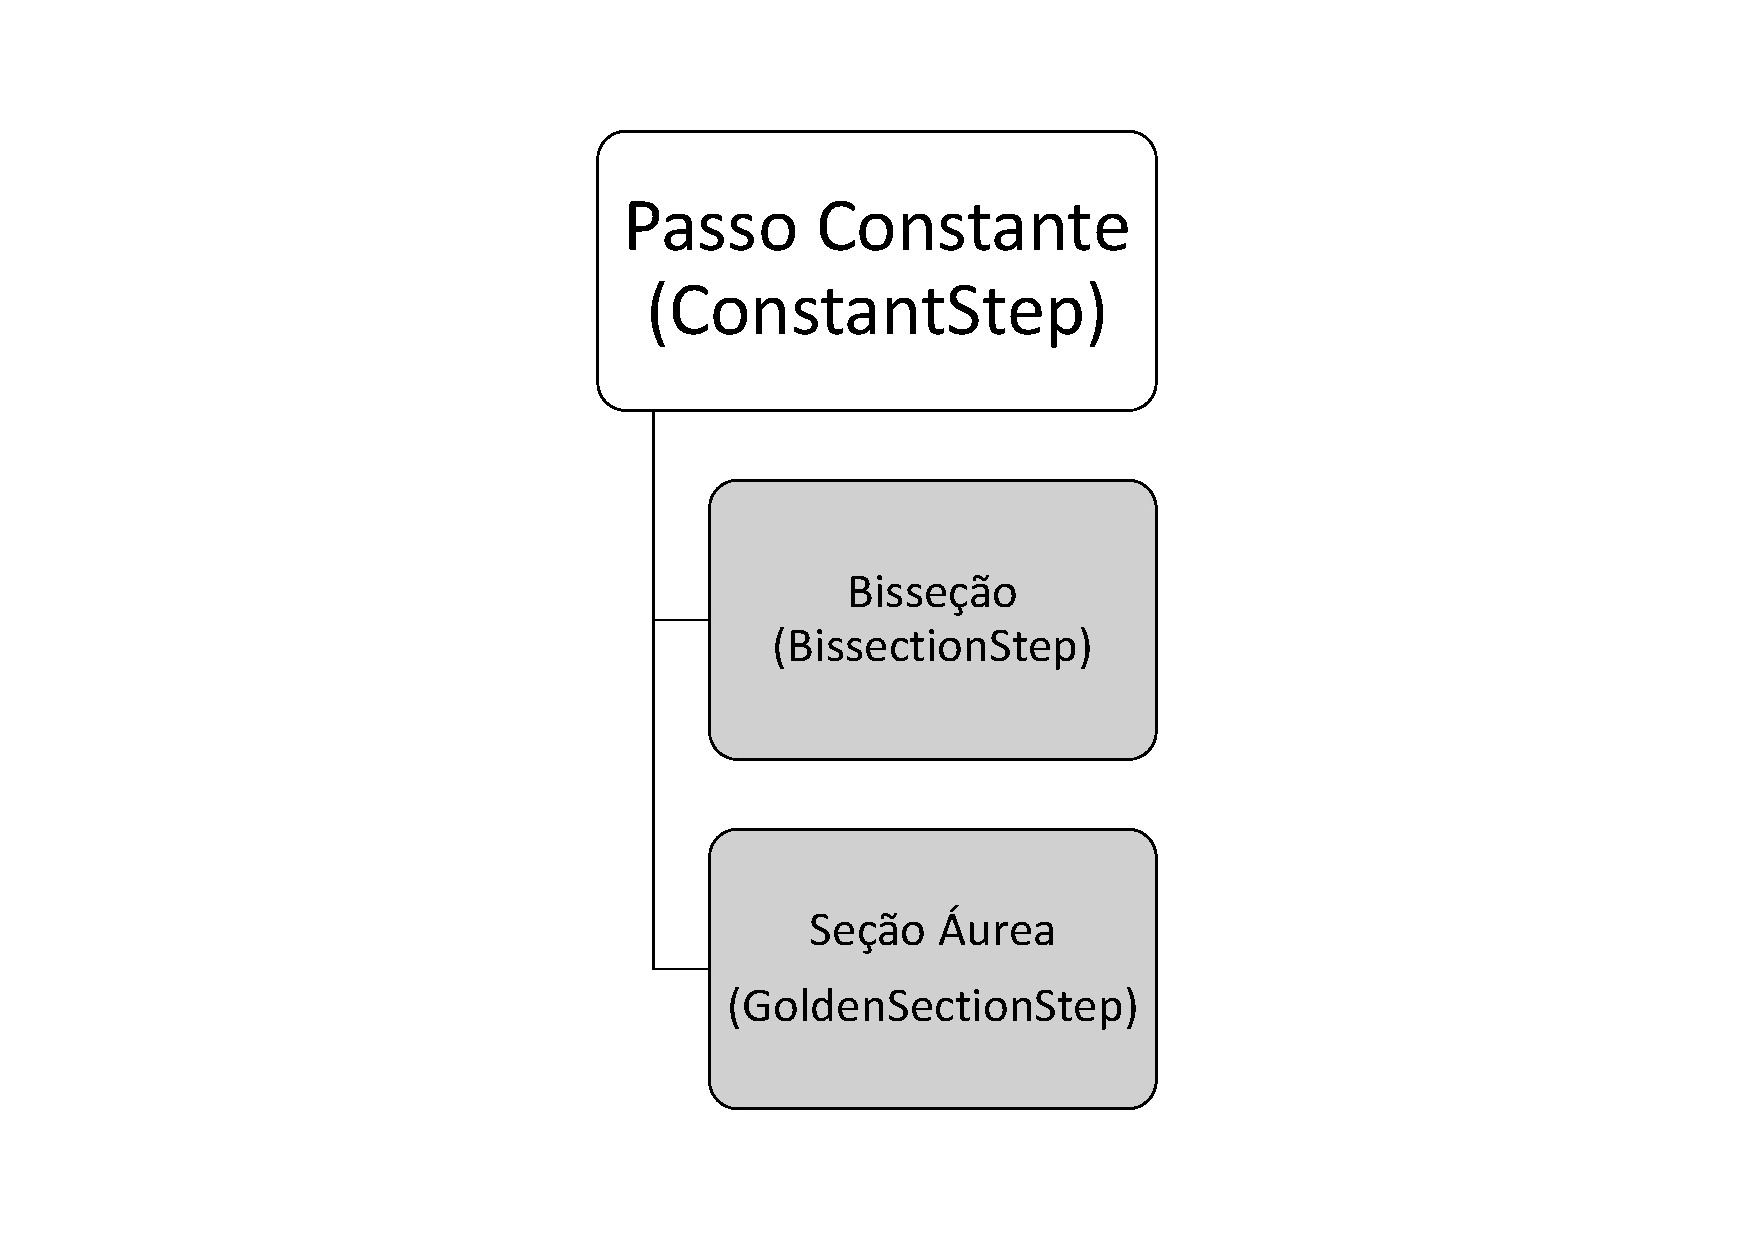
\includegraphics[width=0.8\textwidth]{images/classes.pdf}
  \caption{Estrutura de classes implementada e heranças}
  \label{fig:q1_1}
\end{figure}

O código completo das classes implementadas pode ser visto no arquivo adicionado ao GitHub 
{\tt \href{https://github.com/prj-phcp/MEC2403_Activities/blob/master/packages/steps.py}{steps.py}},
onde a implementação completa das 3 classes está armazenada. Abaixo, para fins de exemplo, é mostrada a implementação da classe de passo constante, da qual todas 
as demais herdam.

\begin{python}
class ConstantStep:
    
    def __init__(self, da):

        self.da = da
        self.aL = None
        self.aU = None
        self.fL = None
        self.fU = None

        self.reset_step()

    def reset_step(self):

        self.aL = 0
        self.aU = self.da
        self.fL =  0.0
        self.fU = -1.0

    def calculate_bounds(self, p_initial, direction, function):

        self.fL = function(*(p_initial + self.aL*direction))
        self.fU = function(*(p_initial + self.aU*direction))

    def __call__(self, p_initial, direction, function):
        
        self.reset_step()
        self.calculate_bounds(p_initial, direction, function)
        while self.fL > self.fU:
            self.aL = self.aU
            self.aU += self.da
            self.calculate_bounds(p_initial, direction, function)
        pend = p_initial + self.aL*direction
        return self.aL, pend
\end{python}

A usabilidade das classes de passo implementadas é feita de forma similar à de uma função graças à implementação de um método {\tt \_\_call\_\_}
em seu corpo. Dessa forma, uma vez declarado o step com seus parâmetros, uma quantidade infinita de passos podem ser dados fornecendo-se como
entrada a função, ponto inicial e direção. Um exemplo do uso dessa classe pode ser visto abaixo.

\begin{python}
import numpy as np
import steps

# Funcao a ser otimizada
def f(x1, x2):
    return np.sin(x1 + x2) + (x1 - x2)**2 - 1.5*x1 + 2.5*x2

# Ponto inicial e direcao
p_inicial = np.array([-2, 3])
d = np.array([1.453, -4.547])

# Instanciando o passo
stp = steps.ConstantStep(da = 0.01)

# Dando o passo
ak, p_final = stp(p_inicial, d, f)
\end{python}

\section{Questão 02}

\subsection{Enunciado}

Utilizando os métodos implementados na questão anterior, testar a sua
implementação encontrando o ponto de mínimo das seguintes funções:

\begin{enumerate}[(a)]
  \item Primeiro Exemplo: \\
        $f(x_1, x_2) = x_1^2 - 3x_1x_2 + 4x_2^2 + x_1 - x_2$ \\
        Ponto inicial: $\mathbf{x^0} = [1, 2]^T$, Direção: $\mathbf{d} = [-1, -2]^T$\label{func:a}
  \item Função de McCormick: \\
        $f(x_1, x_2) = \sin{(x_1 + x_2)} + (x_1 - x_2)^2 - 1.5x_1 + 2.5x_2$ \\
        Ponto inicial: $\mathbf{x^0} = [-2, 3]^T$, Direção: $\mathbf{d} = [1.453, -4.547]^T$\label{func:b}
  \item Função de Himmelblau: \\
        $f(x_1, x_2) = (x_1^2 + x_2 - 11)^2 + (x_1 + x_2^2 - 7)^2$ \\
        Ponto inicial: $\mathbf{x^0} = [0, 5]^T$, Direção: $\mathbf{d} = [3, 1.5]^T$\label{func:c}
\end{enumerate}

Para cada função acima, utilize o MATLAB para desenhar (na mesma figura): as
curvas de nível e o segmento de reta conectando o ponto inicial ao ponto de mínimo.
Adotar tolerância de $10^{-5}$ para verificação da convergência numérica.

\subsection{Solução}

Para executar esse exercício, serão usadas as classes já descritas na Questão 01 (seção \ref{sec:q01}). A biblioteca {\tt matplotlib} do Python será 
novamente usada para gerar os gráficos necessários. Para facilitar a vaisualização, será gerado um gráfico para cada método de cálculo do passo, sendo que 
cada gráfico deverá conter, pelo menos:

\begin{itemize}
  \item As curvas de nível da função a ser estudada
  \item Os pontos iniciais e finais do passo
  \item A direção esperada do passo
  \item Uma seta ou linha ligando os pontos iniciais e finais
  \item O tamanho do passo $\alpha_k$ e coordenadas do ponto final no título do gráfico
\end{itemize}

Um exemplo simples do código que foi usado para gerar os gráficos apresentados neste relatório é apresentado abaixo. 
Em seguida, são apresentadas as seções que mostram os resultados obtidos e alguns comentários a respeito destes.

\begin{python}
step_list   = [steps.ConstantStep(da = 0.01), steps.BissectionStep(da = 0.01, tol = 1e-5), steps.GoldenSectionStep(da = 0.01, tol = 1e-5)]

item = 'a'
x = np.linspace(-3.3, 0.1, 50)
y = np.linspace(3, 5.1, 50)
X, Y = np.meshgrid(x, y)
Z = f(X, Y)

i = 0
for step in step_list:
    i += 1
    t_init = datetime.datetime.now()
    ak, p_final = step(p_inicial, d, f)
    t_final = datetime.datetime.now()
    print(f'Final do passo {i}: ak = {ak}, p_final = [{p_final[0]}, {p_final[1]}].T. Execucao:{t_final - t_init}')
    fig, ax = plt.subplots(1,1, figsize=(5, 5))
    ax.contour(X, Y, Z, cmap='rainbow')
    ax.plot(*p_inicial, 'ro')
    ax.text(p_inicial[0]-0.25, p_inicial[1]+0.04, '$P_{inic}$', color='red')
    ax.plot(*p_final, 'ro')
    ax.text(p_final[0]-0.25, p_final[1]+0.04, '$P_{final}$', color='red')
    ax.quiver(p_inicial[0], p_inicial[1], p_final[0]-p_inicial[0], p_final[1]-p_inicial[1], color='red', angles='xy', scale_units='xy', scale=1)
    ax.quiver(p_inicial[0], p_inicial[1], d[0], d[1], color='black', angles='xy', label='Direcao do passo')
    ax.grid()
    ax.legend()
    ax.set_xlabel('$x_1$')
    ax.set_ylabel('$x_2$')
    ax.set_title(f'$\\alpha_k = {ak:.5f}$, $\mathbf{{P_{{final}}}} = [{p_final[0]:.2f}, {p_final[1]:.2f}]^T$')
    fig.savefig(f'images/q2{item}_{i}.pdf')
\end{python}

\subsubsection{Resultados para a função (\ref{func:a})}

\lipsum[1]

% Figura da funcao a
\begin{figure}
  \centering
  \begin{subfigure}[b]{0.32\textwidth}
      \centering
      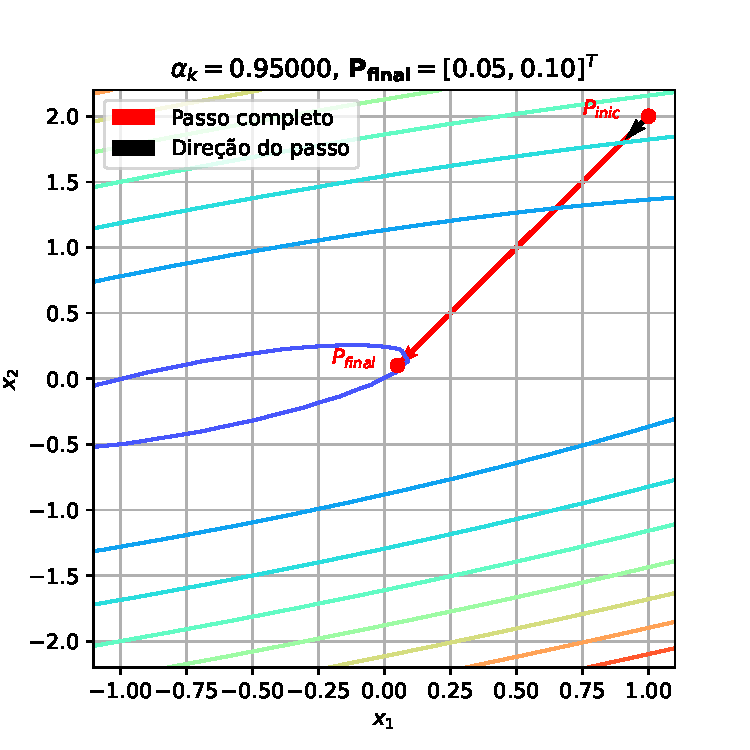
\includegraphics[width=\textwidth]{images/q2a_1.pdf}
      \caption{Passo constante}
      \label{fig:q2a_1}
  \end{subfigure}
  \hfill
  \begin{subfigure}[b]{0.32\textwidth}
      \centering
      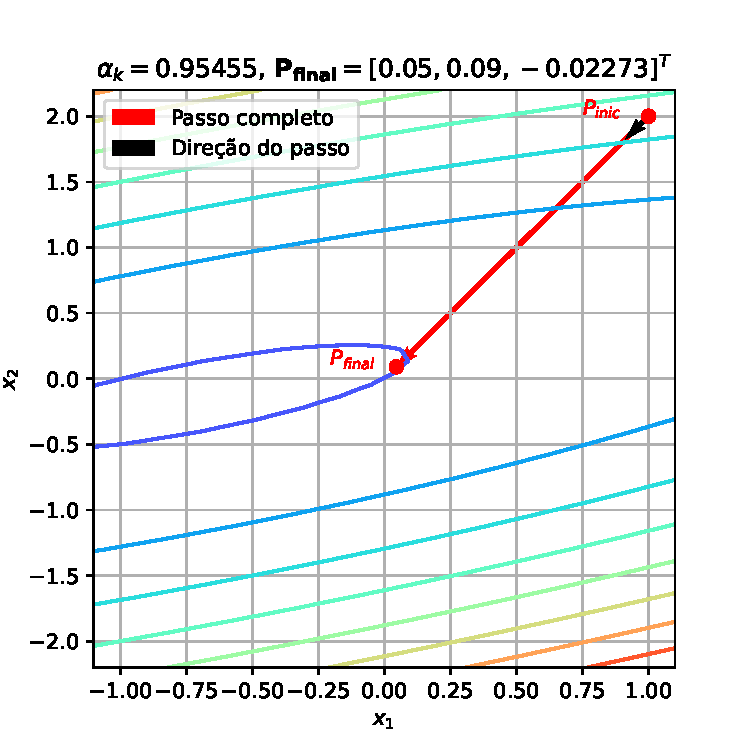
\includegraphics[width=\textwidth]{images/q2a_2.pdf}
      \caption{Bisseção}
      \label{fig:q2a_2}
  \end{subfigure}
  \hfill
  \begin{subfigure}[b]{0.32\textwidth}
      \centering
      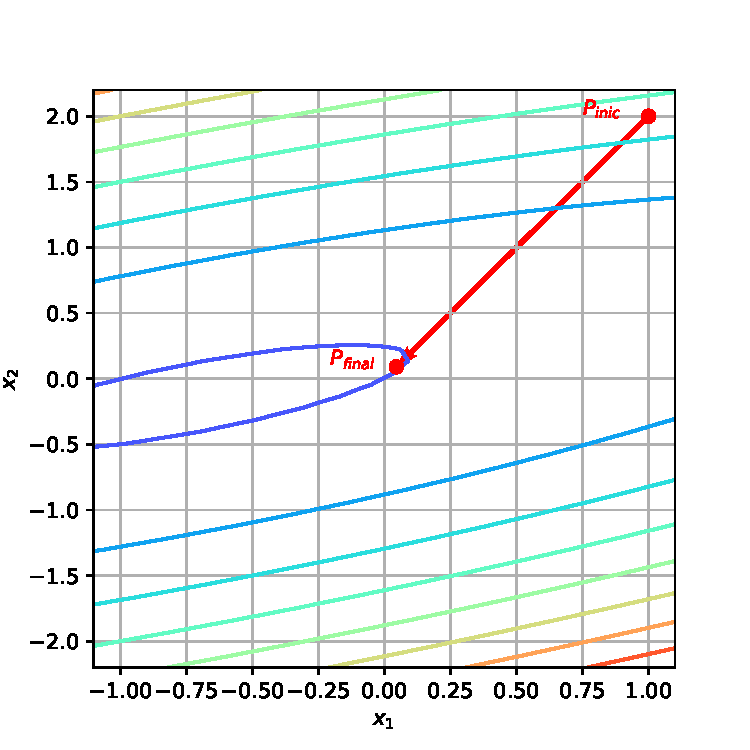
\includegraphics[width=\textwidth]{images/q2a_3.pdf}
      \caption{Razão áurea}
      \label{fig:q2a_3}
  \end{subfigure}
  \caption{Resultados para a função (\ref{func:a}) caso com diferentes métodos}
  \label{fig:q2a}
\end{figure}

\subsubsection{Resultados para a função (\ref{func:b})}

\lipsum[1]

% Figura da funcao b
\begin{figure}
  \centering
  \begin{subfigure}[b]{0.32\textwidth}
      \centering
      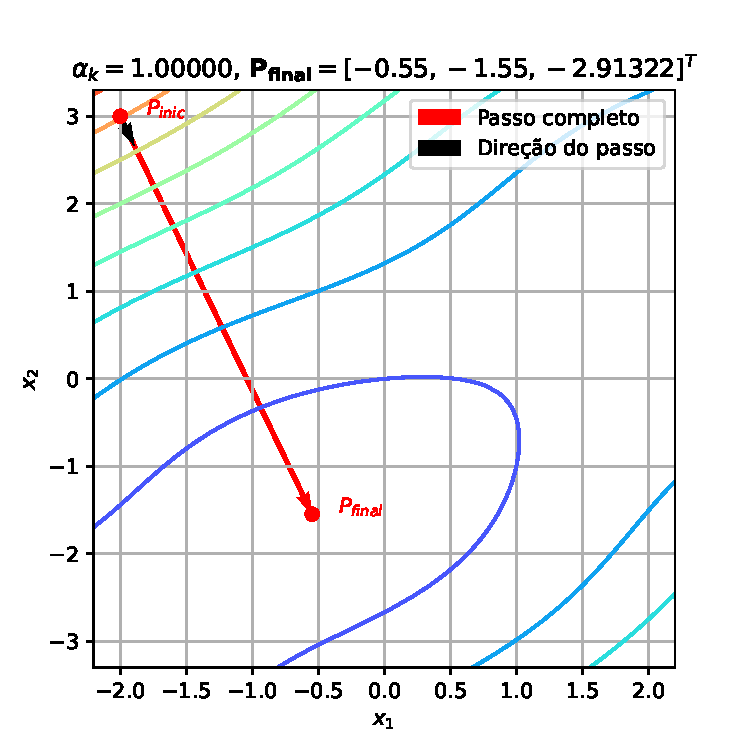
\includegraphics[width=\textwidth]{images/q2b_1.pdf}
      \caption{Passo constante}
      \label{fig:q2b_1}
  \end{subfigure}
  \hfill
  \begin{subfigure}[b]{0.32\textwidth}
      \centering
      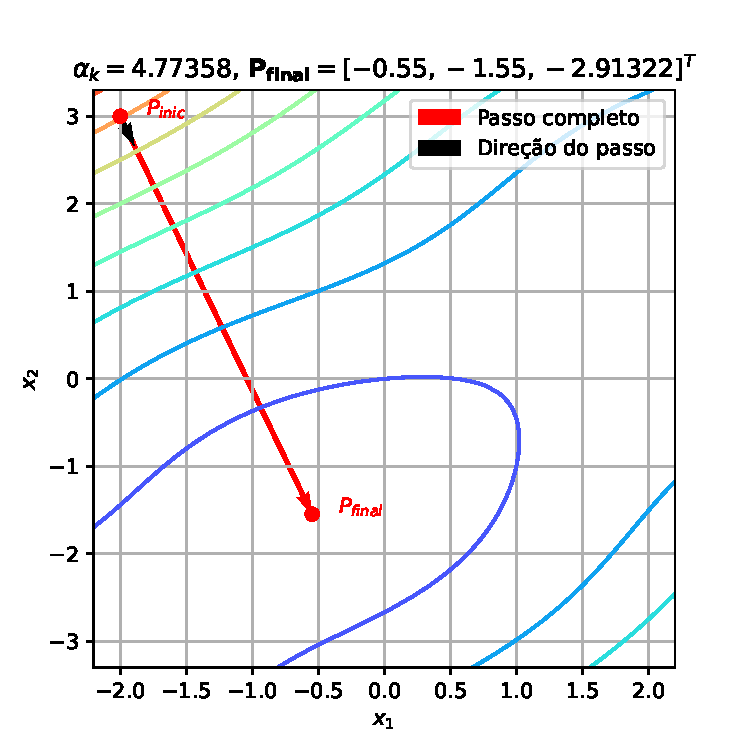
\includegraphics[width=\textwidth]{images/q2b_2.pdf}
      \caption{Bisseção}
      \label{fig:q2b_2}
  \end{subfigure}
  \hfill
  \begin{subfigure}[b]{0.32\textwidth}
      \centering
      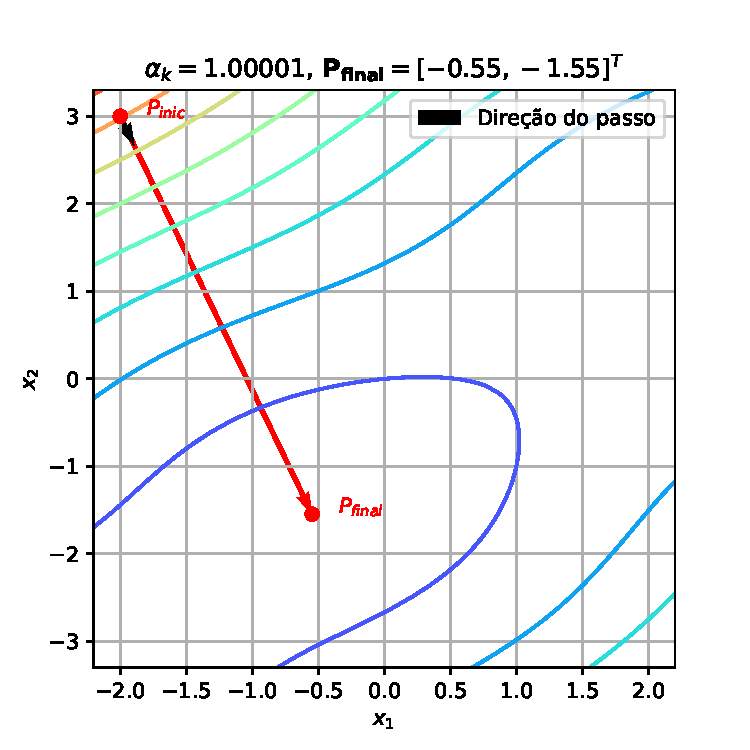
\includegraphics[width=\textwidth]{images/q2b_3.pdf}
      \caption{Razão áurea}
      \label{fig:q2b_3}
  \end{subfigure}
     \caption{Resultados para a função (\ref{func:b}) com diferentes métodos}
     \label{fig:q2b}
\end{figure}

\subsubsection{Resultados para a função (\ref{func:c})}

\lipsum[1]

% Figura da funcao c
\begin{figure}
  \centering
  \begin{subfigure}[b]{0.32\textwidth}
      \centering
      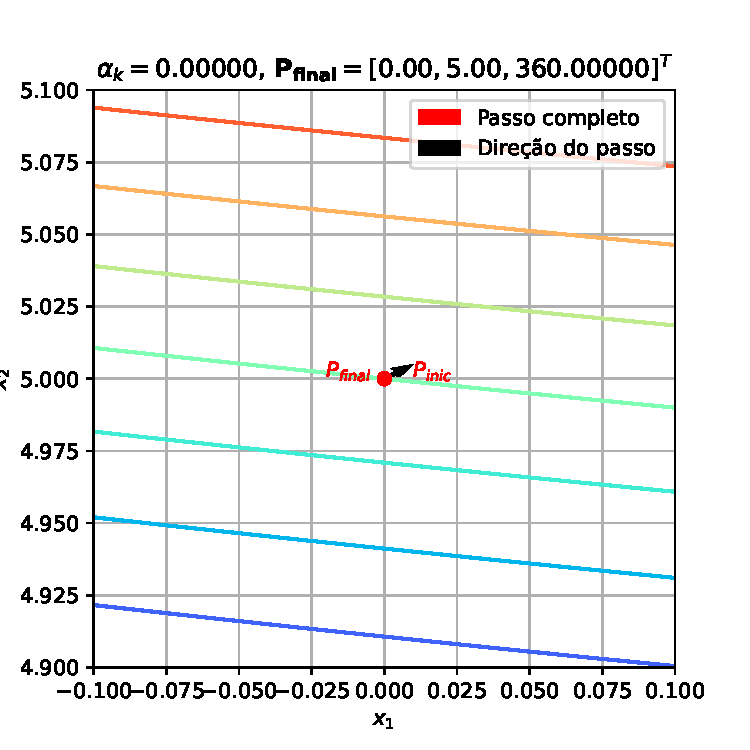
\includegraphics[width=\textwidth]{images/q2c_1.pdf}
      \caption{Passo constante}
      \label{fig:q2c_1}
  \end{subfigure}
  \hfill
  \begin{subfigure}[b]{0.32\textwidth}
      \centering
      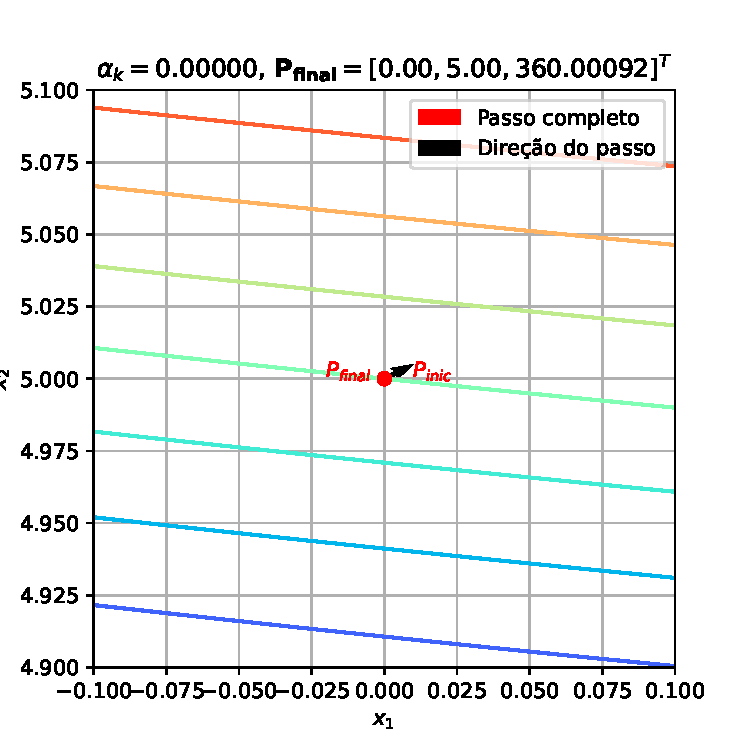
\includegraphics[width=\textwidth]{images/q2c_2.pdf}
      \caption{Bisseção}
      \label{fig:q2c_2}
  \end{subfigure}
  \hfill
  \begin{subfigure}[b]{0.32\textwidth}
      \centering
      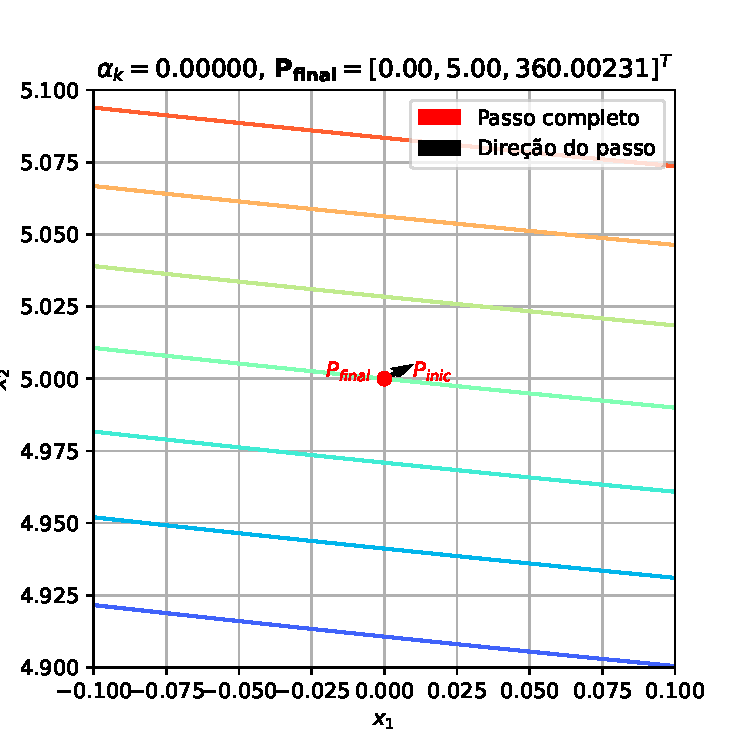
\includegraphics[width=\textwidth]{images/q2c_3.pdf}
      \caption{Razão áurea}
      \label{fig:q2c_3}
  \end{subfigure}
     \caption{Resultados para a função (\ref{func:c}) com diferentes métodos}
     \label{fig:q2c}
\end{figure}

% Figura da funcao c - reversa
\begin{figure}
  \centering
  \begin{subfigure}[b]{0.32\textwidth}
      \centering
      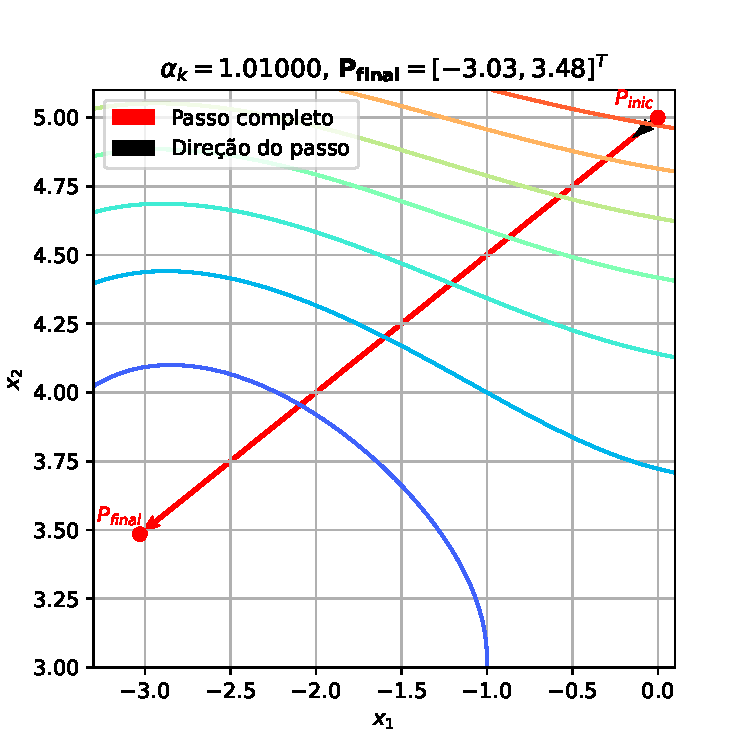
\includegraphics[width=\textwidth]{images/q2c2_1.pdf}
      \caption{Passo constante}
      \label{fig:q2c2_1}
  \end{subfigure}
  \hfill
  \begin{subfigure}[b]{0.32\textwidth}
      \centering
      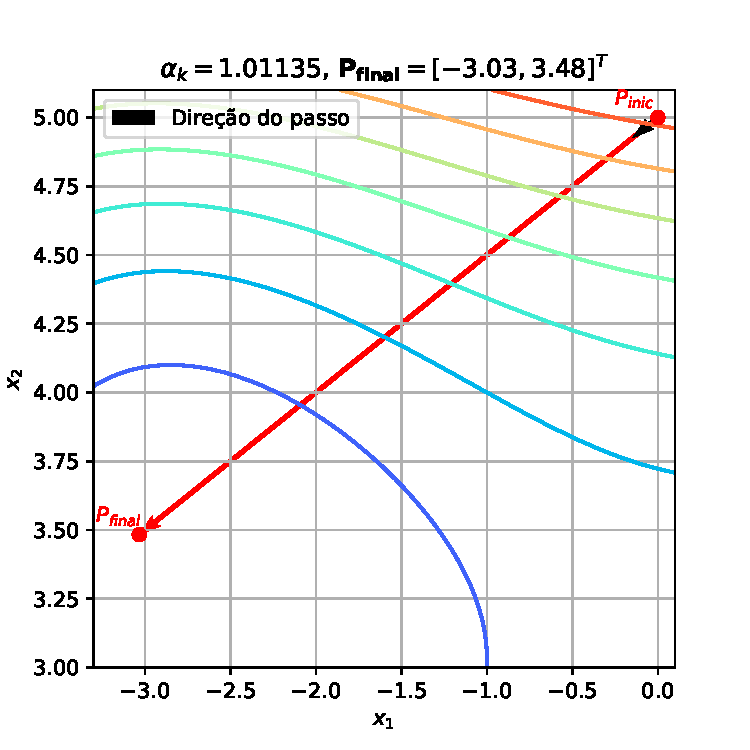
\includegraphics[width=\textwidth]{images/q2c2_2.pdf}
      \caption{Bisseção}
      \label{fig:q2c2_2}
  \end{subfigure}
  \hfill
  \begin{subfigure}[b]{0.32\textwidth}
      \centering
      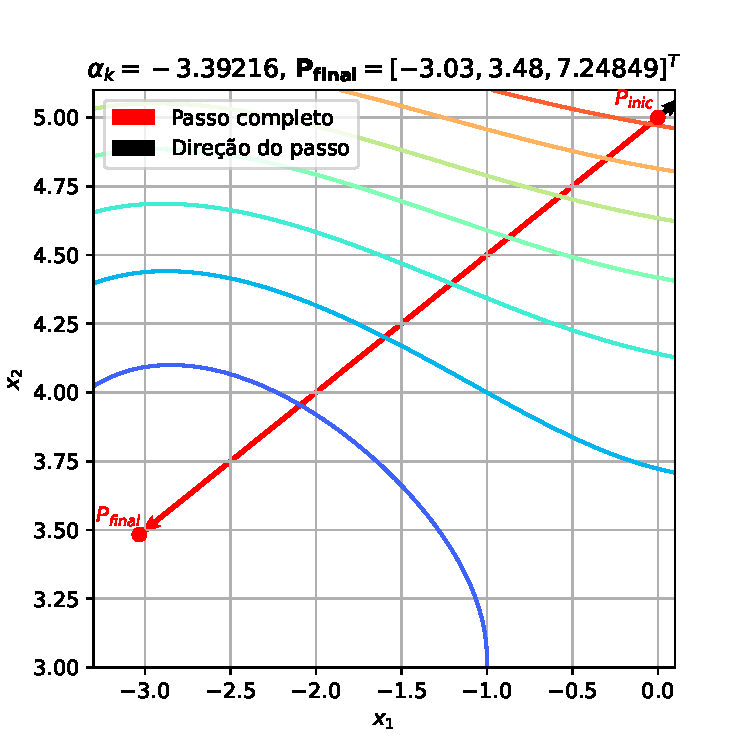
\includegraphics[width=\textwidth]{images/q2c2_3.pdf}
      \caption{Razão áurea}
      \label{fig:q2c2_3}
  \end{subfigure}
     \caption{Resultados para a função (\ref{func:c}) com diferentes métodos (revertendo a direção)}
     \label{fig:q2c2}
\end{figure}

%%%%%%%%%%%%%%%%%%%%%%%%%%%%%%%%%%%%%%%%%%%%%%%%%%%

\bibliographystyle{apalike}
\bibliography{export}

\end{document}